% Created 2023-10-07 Sat 13:45
% Intended LaTeX compiler: pdflatex
\documentclass[11pt]{article}
\usepackage[utf8]{inputenc}
\usepackage[T1]{fontenc}
\usepackage{graphicx}
\usepackage{longtable}
\usepackage{wrapfig}
\usepackage{rotating}
\usepackage[normalem]{ulem}
\usepackage{amsmath}
\usepackage{amssymb}
\usepackage{capt-of}
\usepackage{hyperref}
\usepackage{color}
\usepackage{listings}
\author{Biggie Dickus}
\date{\today}
\title{}
\hypersetup{
 pdfauthor={Biggie Dickus},
 pdftitle={},
 pdfkeywords={},
 pdfsubject={},
 pdfcreator={Emacs 30.0.50 (Org mode 9.6.7)}, 
 pdflang={English}}

% Setup for code blocks [1/2]

\usepackage{fvextra}

\fvset{%
  commandchars=\\\{\},
  highlightcolor=white!95!black!80!blue,
  breaklines=true,
  breaksymbol=\color{white!60!black}\tiny\ensuremath{\hookrightarrow}}

% Make line numbers smaller and grey.
\renewcommand\theFancyVerbLine{\footnotesize\color{black!40!white}\arabic{FancyVerbLine}}

\usepackage{xcolor}

% In case engrave-faces-latex-gen-preamble has not been run.
\providecolor{EfD}{HTML}{f7f7f7}
\providecolor{EFD}{HTML}{28292e}

% Define a Code environment to prettily wrap the fontified code.
\usepackage[breakable,xparse]{tcolorbox}
\DeclareTColorBox[]{Code}{o}%
{colback=EfD!98!EFD, colframe=EfD!95!EFD,
  fontupper=\footnotesize\setlength{\fboxsep}{0pt},
  colupper=EFD,
  IfNoValueTF={#1}%
  {boxsep=2pt, arc=2.5pt, outer arc=2.5pt,
    boxrule=0.5pt, left=2pt}%
  {boxsep=2.5pt, arc=0pt, outer arc=0pt,
    boxrule=0pt, leftrule=1.5pt, left=0.5pt},
  right=2pt, top=1pt, bottom=0.5pt,
  breakable}

% Support listings with captions
\usepackage{float}
\floatstyle{plain}
\newfloat{listing}{htbp}{lst}
\newcommand{\listingsname}{Listing}
\floatname{listing}{\listingsname}
\newcommand{\listoflistingsname}{List of Listings}
\providecommand{\listoflistings}{\listof{listing}{\listoflistingsname}}


% Setup for code blocks [2/2]: syntax highlighting colors

\newcommand\efstrut{\vrule height 2.1ex depth 0.8ex width 0pt}
\definecolor{EFD}{HTML}{000000}
\definecolor{EfD}{HTML}{ffffff}
\newcommand{\EFD}[1]{\textcolor{EFD}{#1}} % default
\definecolor{EFh}{HTML}{7f7f7f}
\newcommand{\EFh}[1]{\textcolor{EFh}{#1}} % shadow
\definecolor{EFsc}{HTML}{228b22}
\newcommand{\EFsc}[1]{\textcolor{EFsc}{\textbf{#1}}} % success
\definecolor{EFw}{HTML}{ff8e00}
\newcommand{\EFw}[1]{\textcolor{EFw}{\textbf{#1}}} % warning
\definecolor{EFe}{HTML}{ff0000}
\newcommand{\EFe}[1]{\textcolor{EFe}{\textbf{#1}}} % error
\definecolor{EFc}{HTML}{b22222}
\newcommand{\EFc}[1]{\textcolor{EFc}{#1}} % font-lock-comment-face
\definecolor{EFcd}{HTML}{b22222}
\newcommand{\EFcd}[1]{\textcolor{EFcd}{#1}} % font-lock-comment-delimiter-face
\definecolor{EFs}{HTML}{8b2252}
\newcommand{\EFs}[1]{\textcolor{EFs}{#1}} % font-lock-string-face
\definecolor{EFd}{HTML}{8b2252}
\newcommand{\EFd}[1]{\textcolor{EFd}{#1}} % font-lock-doc-face
\definecolor{EFm}{HTML}{008b8b}
\newcommand{\EFm}[1]{\textcolor{EFm}{#1}} % font-lock-doc-markup-face
\definecolor{EFk}{HTML}{9370db}
\newcommand{\EFk}[1]{\textcolor{EFk}{#1}} % font-lock-keyword-face
\definecolor{EFb}{HTML}{483d8b}
\newcommand{\EFb}[1]{\textcolor{EFb}{#1}} % font-lock-builtin-face
\definecolor{EFf}{HTML}{0000ff}
\newcommand{\EFf}[1]{\textcolor{EFf}{#1}} % font-lock-function-name-face
\definecolor{EFv}{HTML}{a0522d}
\newcommand{\EFv}[1]{\textcolor{EFv}{#1}} % font-lock-variable-name-face
\definecolor{EFt}{HTML}{228b22}
\newcommand{\EFt}[1]{\textcolor{EFt}{#1}} % font-lock-type-face
\definecolor{EFo}{HTML}{008b8b}
\newcommand{\EFo}[1]{\textcolor{EFo}{#1}} % font-lock-constant-face
\definecolor{EFwr}{HTML}{ff0000}
\newcommand{\EFwr}[1]{\textcolor{EFwr}{\textbf{#1}}} % font-lock-warning-face
\newcommand{\EFnc}[1]{#1} % font-lock-negation-char-face
\definecolor{EFpp}{HTML}{483d8b}
\newcommand{\EFpp}[1]{\textcolor{EFpp}{#1}} % font-lock-preprocessor-face
\newcommand{\EFrc}[1]{\textbf{#1}} % font-lock-regexp-grouping-construct
\newcommand{\EFrb}[1]{\textbf{#1}} % font-lock-regexp-grouping-backslash
\newcommand{\EFob}[1]{#1} % org-block
\definecolor{EFhn}{HTML}{008b8b}
\newcommand{\EFhn}[1]{\textcolor{EFhn}{#1}} % highlight-numbers-number
\definecolor{EFhq}{HTML}{9370db}
\newcommand{\EFhq}[1]{\textcolor{EFhq}{#1}} % highlight-quoted-quote
\definecolor{EFhs}{HTML}{008b8b}
\newcommand{\EFhs}[1]{\textcolor{EFhs}{#1}} % highlight-quoted-symbol
\definecolor{EFrda}{HTML}{707183}
\newcommand{\EFrda}[1]{\textcolor{EFrda}{#1}} % rainbow-delimiters-depth-1-face
\definecolor{EFrdb}{HTML}{7388d6}
\newcommand{\EFrdb}[1]{\textcolor{EFrdb}{#1}} % rainbow-delimiters-depth-2-face
\definecolor{EFrdc}{HTML}{909183}
\newcommand{\EFrdc}[1]{\textcolor{EFrdc}{#1}} % rainbow-delimiters-depth-3-face
\definecolor{EFrdd}{HTML}{709870}
\newcommand{\EFrdd}[1]{\textcolor{EFrdd}{#1}} % rainbow-delimiters-depth-4-face
\definecolor{EFrde}{HTML}{907373}
\newcommand{\EFrde}[1]{\textcolor{EFrde}{#1}} % rainbow-delimiters-depth-5-face
\definecolor{EFrdf}{HTML}{6276ba}
\newcommand{\EFrdf}[1]{\textcolor{EFrdf}{#1}} % rainbow-delimiters-depth-6-face
\definecolor{EFrdg}{HTML}{858580}
\newcommand{\EFrdg}[1]{\textcolor{EFrdg}{#1}} % rainbow-delimiters-depth-7-face
\definecolor{EFrdh}{HTML}{80a880}
\newcommand{\EFrdh}[1]{\textcolor{EFrdh}{#1}} % rainbow-delimiters-depth-8-face
\definecolor{EFrdi}{HTML}{887070}
\newcommand{\EFrdi}[1]{\textcolor{EFrdi}{#1}} % rainbow-delimiters-depth-9-face
\begin{document}

\tableofcontents

\section{Idea generale}
\label{sec:orgdc2c950}
ci sono molti modi di interpretare/compilare/eseguire un linguaggio per fottere un attimo i disegni a \href{https://craftinginterpreters.com/a-map-of-the-territory.html}{questo libro}\footnote{di cui ho letto mezzo capitolo prima di rompermi il cazzo che non potevo scaricare il pdf, perchè sono un bambino viziato}
\begin{center}
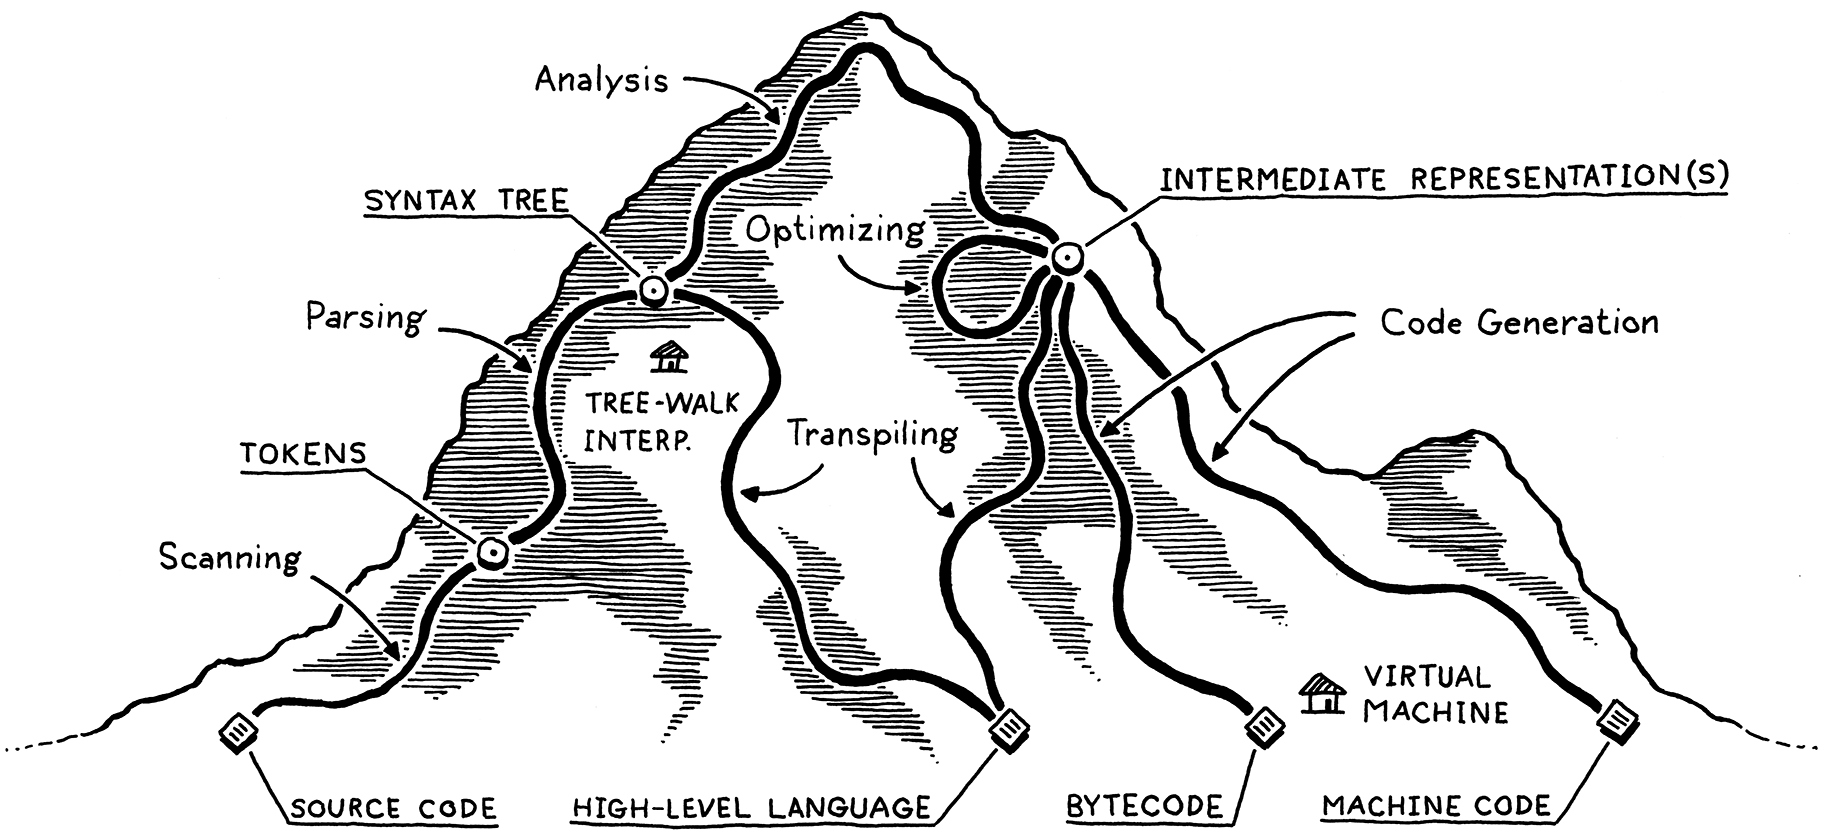
\includegraphics[width=.9\linewidth]{./mountain.png}
\end{center}
quello che intendo fare, per mera facilità di interpretazione, è un \texttt{Tree-Walk Interpreter} (quella casetta messa a cazzo in mezzo alla montagna)

sarebbe a dire
\begin{itemize}
\item prendi il codice
\item capisci che cazzo di struttura ha
\item runna brutalmente dalla struttura senza neanche pensarci di usarla per transpiling \&Co.
\end{itemize}

ognino di questi passi ha come input l'output dello step precedente
\begin{itemize}
\item la prima parte ha come output il codice
\item capire la struttura ha come input il codice e come output la struttura
\item runnare la struttura ha come input la struttura
\end{itemize}

quindi rappresentiamo tutto malissimo con un
\begin{verbatim}
codice -> struttura -> esecuzione struttura
\end{verbatim}

si illustrano mo' queste fasi del programma

\section{Prendi il codice}
\label{sec:org7b5900b}
abbiamo due modi per prendere il codice, il primo è il classico "leggi un file"
a fini di testing e per certi use case vorrei però che fosse anche possibile leggere codice lisp da una stringa messa nel codice java

per abusare un po' l'uml possiamo metterla in questo modo
\begin{center}
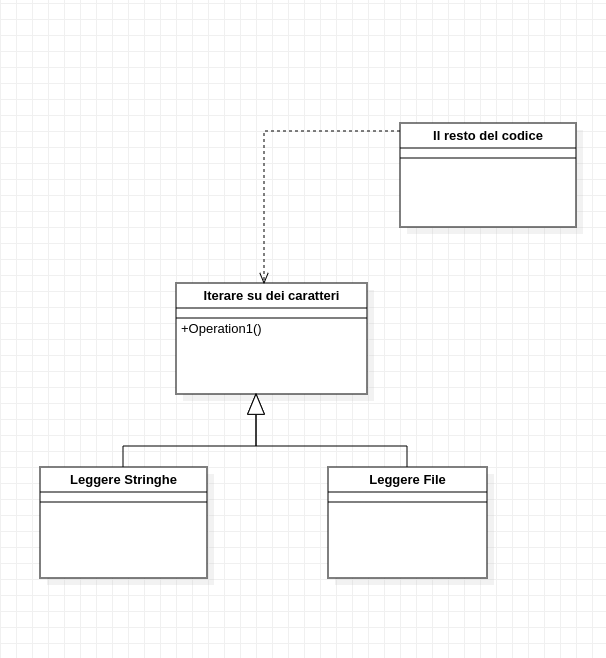
\includegraphics[width=.9\linewidth]{./chars.png}
\end{center}

\section{Struttura del codice}
\label{sec:orgdb2450a}
per semplificarci la vita, capire la struttura del codice qui si divide in 2 passi
\begin{itemize}
\item tokenizing
\item il resto
\end{itemize}

\subsection{Tokenizing}
\label{sec:orgaaa828a}
con tokenizing si intende prendere la stringa di codice e dividerla in quei pezzi che hanno effettivamente un significato, quindi un
\begin{Code}
\begin{Verbatim}
\color{EFD}\EFs{"for(int i=1; i<max; ++i) \{res = res*i;\}"}
\end{Verbatim}
\end{Code}
viene diviso nella sequenza
\begin{Code}
\begin{Verbatim}
\color{EFD}\EFrda{\{}\EFs{"for"}, \EFs{"("}, \EFs{"int"}, \EFs{"i"}, \EFs{"="}, \EFs{"1"}, \EFs{";"}, \EFs{"i"}, \EFs{"<"}, \EFs{"max"}, \EFs{";"}, \EFs{"++"}, \EFs{"i"}, \EFs{")"},
        \EFs{"\{"}, \EFs{"res"}, \EFs{"="}, \EFs{"res"}, \EFs{"*"}, \EFs{"i"}, \EFs{";"}, \EFs{"\}"}\EFrda{\}}
\end{Verbatim}
\end{Code}

\subsection{Il resto}
\label{sec:org49ebe70}
il resto consiste nel prendere la sequenza di sottostringhe data dal tokenizer e usarla per costruire il dannatissimo \emph{Albero del Codice}.

\subsubsection{Perché è una cazzata farlo in lisp}
\label{sec:orgbcad72c}
qui è dove lisp inizia a tirare di brutto, perchè l'albero del codice è definito solo ed interamete dalle parentesi, per quanto "prendi stringa di parentesi e costruisci l'albero che definisce" sia un po' stronzo, non è niente rispetto a quanto ci vuole a fare parsing di linguaggio più comuni.

\subsubsection{Perchè non è una cazzata farlo in java}
\label{sec:orgecd541b}
se pensi in java potresi avere anche solo un
\begin{Code}
\begin{Verbatim}
\color{EFD}x + 2;
\end{Verbatim}
\end{Code}
che ti obbligherebbe a dover
\begin{itemize}
\item capire che \texttt{x + 2} è un'espressione
\item capire che è l'applicazione dell'operatore \texttt{+} a \texttt{x} e \texttt{2}
\end{itemize}

non troppo bastardo, ma metti un
\begin{Code}
\begin{Verbatim}
\color{EFD}x + 2 * y;
\end{Verbatim}
\end{Code}
qui dobbiamo
\begin{itemize}
\item capire che è un'espressoine
\item capire che \texttt{+} e \texttt{*} sono gli operatori
\item andare di precedenza di operatori per fare \texttt{x + (2 * y)}
\end{itemize}

visto che ho già abbastanza traumi di mio con la precedenza di operatori, e che non voglio capire come implementarla, direi di evitare

poi andiamo a casi come
\begin{Code}
\begin{Verbatim}
\color{EFD}\EFk{if}\EFrda{(}x>10\EFrda{)}
    \EFk{return} x;
\EFk{else}
    \EFk{return} x+2;
\end{Verbatim}
\end{Code}

e onestamente, direi di evitare

\section{Esecuzione della struttura}
\label{sec:org9085583}
\begin{quote}
\textbf{NOTA}: di solito per capire un minimo cosa cazzo sto facendo devo iniziare a implementarlo.
Questa parte non l'ho ancora fatta, quindi la discussione potrebbero essere un po' confusa.
C'è evaluator.org nella cartella docs/ (quella sopra questa) con un po' di dettagli extra, ma sono più note che mi sono fatto per me, quindi potrebbe far cagare altrettanto il cazzo, scusate
\end{quote}

ora che abbiamo la struttura (di lista) del codice possiamo pensare a come eseguirla, prendiamo, come esempio di questa sezione, l'espressione
\begin{Code}
\begin{Verbatim}
\color{EFD}\EFrda{(}\EFk{if} \EFrdb{(}= x 10\EFrdb{)}
    \EFrdb{(}print \EFs{"fa 10"}\EFrdb{)}
  \EFrdb{(}print \EFs{"non fa 10"}\EFrdb{)}\EFrda{)}
\end{Verbatim}
\end{Code}

per eseguire questa espressione dobbiamo
\begin{itemize}
\item capire che è un \texttt{if}
\item ora che sappiamo che è un \texttt{if}
\begin{itemize}
\item capire quale sia la condizione da controllare
\item capire quale parte del \texttt{then}
\item capire quale quella dell'\texttt{else}
\end{itemize}
\item determinare se la condizione da controllare è vera
\begin{itemize}
\item se lo è esegui la parte del \texttt{then}
\item altrimenti quella dell'\texttt{else}
\end{itemize}
\end{itemize}

detta in modo un po' meno stronzo
\begin{itemize}
\item capire che è un \texttt{if}
\item capito che è un \texttt{if}, determinare le parti dell'\texttt{if}, "costruire" l'\texttt{if}, per così dire
\item costruito l'if, eseguirlo
\end{itemize}

sono sotto illustrate le tre parti in questione

\begin{quote}
sotto non gli ho ancora illustarati perchè devo capire meglio come farli e come documentarli
\end{quote}
\end{document}